\documentclass[
    Title      = 你的论文标题,
    Institute  = 你的学院,
    Major      = 你的专业,
    Name       = 你的名字,
    StudentId  = 你的学号,
    Supervisor = 你的指导老师,
    SubmitDate = 提交日期,
]{scutthesis}

\usepackage{lipsum}

\begin{document}

\cover
\makestatement

\prevstyle
\begin{cabstract}
    这是一个华南理工个大学本科毕业论文 \LaTeX 模板,根据华南理工大学 2021 届本科毕业生论文模板 Word 版制作而成。
    它是个人作品,不代表官方立场,所以请自行承担可能发生的任何后果。
    其中对Word模板的格式要求,已在文档中说明,若日后不满足新的格式要求,欢迎在 Github 提出 issue 或发送 pull request。

    此文档主要有三章,一为模板的格式说明,二为环境搭建,三为如何编写。

    若此模板对你起到了帮助,麻烦在 Github 给个 Star。
    \ckeywords{\LaTeX 模板;华南理工大学;本科毕设}
\end{cabstract}

\begin{eabstract}
    This is a \LaTeX~template for South China University of Technology undergraduate thesis, and it is made upon Word version of the 2021 undergraduate thesis template of South China University of Technology.
    It is a personal work and does not represent the official template.
    Please bear any consequences that may occur.
    The format requirements for the Word template have been explained in the document.
    If the new format requirements are not met in the future, you are welcome to open an issue or send a pull request on Github.

    There is mainly three chapters in this document, one is the format description of the template, the second is the environment construction, and the third is how to write.

     If this template helps you, please give me a star on Github.
    \ekeywords{\LaTeX~template, South China University of Technology, graduation project}
\end{eabstract}

\begin{spacing}{1.5}
    \clearpage
    {
      \hypersetup{
          linkbordercolor=black,
          linkcolor=black,
      }
      \addcontentsline{toc}{chapter}{目录}
      \tableofcontents
    }

    \clearpage
    \mainstyle
    \chapter{格式说明}

\section{纸张}

标准 A4 纸,上下左右页面边距为 25mm。

论文封面(底)、摘要和目录实行单面打印;
论文主体部分(引言、正文、结论、参考文献、附录)实行双面打印。

\section{页眉页脚}

\subsection{页眉}

页眉标注从论文主体部分(绪论、正文、结论)开始。
页眉分奇、偶页标注,其中偶数页的页眉为“华南理工大学学士学位论文”;
奇数页的页眉为章序及章标题。
页眉的上边距为 15mm,在版心上边线加一行 1.0 磅粗的实线,其上居中打印页眉;

\subsection{页脚}

论文页码从主体部分(绪论、正文、结论)开始,直至“参考文献、附录、致谢”结束,用五号阿拉伯数字编连续码,页码位于页脚居中。
摘要、目录、图表清单、主要符号表用五号罗马数字编连续码,页码位于页脚居中。
封面不编入页码。
页脚的下边距为 15mm。

\section{封面}

校徽:高度 2.75 cm。

类型:初号,黑体,居中。

标题:二号,黑体,加粗,居中。

信息:小三号,宋体,加粗,两端对齐。


\section{摘要}

\subsection{中文}

标题:小二号,黑体,居中,单倍行距,段前、段后各 0.5 行,两字中间空 2 字符。

正文:小四号,宋体,1.5 倍行距,段首行空两个汉字。

关键词标题:小四号,黑体,不缩进。

关键词内容:小四号,宋体。关键词之间用 ; 隔开,最后一个关键词不用分隔符。

\subsection{英文}

标题:小二号,Times New Roman 字体,居中,单倍行距,段前、段后各 0.5 行。

正文:小四号,Times New Roman 字体,1.5 倍行距,段首行空两个汉字,两端对齐。

关键词标题:小四号,Times New Roman 字体,不缩进,加粗。

关键词内容:小四号,Times New Roman 字体,关键词之间用 , 隔开,最后一个关键词不用分隔符。

\section{目录}

标题:小二号,黑体,居中,两字之间空 2 字符。

摘要、Abstract、目录、各章标题、结论、参考文献、致谢等:黑体,四号。

其余:宋体,小四号,行距 1.5 倍

\section{标题与正文}

各章标题:同中文摘要标题,章节序号与标题之间空一字符。

总结标题、参考文献标题、致谢标题:同中文摘要标题。

各节一级标题:黑体,小三号,居左,单倍行距,段前、段后各 0.5 行。

各节二级标题:黑体,四号,居左,单倍行距,段前、段后各 0.5 行。

各节二级标题:黑体,小四号,居左,单倍行距,段前、段后各 0.5 行。

正文:1.5 倍行距,
中文:宋体,小四号,每段首行空 2 个汉字;
字母和阿拉伯数字(含引用的数字):Times New Roman 字体,小四号。

\section{公式}

公式一般居中书写,序号按章编排,如本公式为第二章第一个公式,则序号为 (2-1)。

\section{表}

标题:位于表的上方,一般居中,宋体,五号。

序号:按章编排,如第四章第一个表,则序号为“表 4-1”,序号与文字描述之间空一格。

网格:表格不加左、右列线。

内容:表内数字空缺的格内加 “—” 字线。中文使用宋体,五号。

\section{图}

标题:位于图的下方,一般居中,宋体,五号。

序号:按章编排,如第四章第一个图,则序号为“图 4-1”,序号与文字描述之间空一格。

子图的需要用 a)、b)等表示。

\section{注释}

论文中有个别名称或情况需要解释时,可加注说明,注释可用页末注(将注文放在加注页稿纸的下端)或篇末注(将全部注文几种在文章末尾),而不可用行中注(即注文夹在正文中)。


\section{附录}

标题:同中文摘要标题。

正文:同摘要中文正文。

\section{参考文献}

标题:同中文摘要标题。

正文:同摘要中文正文。

\begin{description}
    \item[专著:] [序号] 作者名. 书名[M]. 出版地:出版单位,出版年:引文页码. 
    \item[期刊:] [序号] 作者名. 题名[J]. 刊名,年,卷号(期号):所引用的文献在期刊中的起止页码. 
    \item[报纸:] [序号] 作者名. 题名[N]. 报刊名,年-月-日(版次) .
    \item[论文集:] 析出文献主要责任者.析出文献题名[A].原文献主要责任者(可选).原文献题名[C].出版地:出版者,出版年.起止页码.
    \item[专利:] [序号]专利所有者.专利题名[P].专利国别:专利号,发布日期.
    \item[技术标准:] [序号]标准代号,标准名称[S].出版地:出版者,出版年.
    \item[报告:] [序号]作者.文献题名[R].报告地:报告会主办单位,年份.
    \item[电子文献:] [序号]作者.电子文献题名[文献类型/载体类型].文献网址或出处,发表或更新日期/引用日期(任选). 
    \item[学位论文:] [序号] 作者名. 题名[D]. 授予单位所在地:授予单位,授予年.
    \item[外文参考文献:] 按语言所在国学术界通行的格式
\end{description}

参考文献作者三名以内的全部列出,四名以上的列前三名,中文后加“等”,英文后加“et al”。
    \chapter{环境配置}

本章只是简单介绍一下环境的配置,分为云平台和本地平台两部分。
云平台无需配置,直接使用。
本地部分只是粗略介绍,细节部分可自行搜索获得。
欢迎各位来补充。

\section{云平台}

本模板已经在 \href{https://www.overleaf.com}{OverLeaf}\footnote{一个在线的 \LaTeX 平台} 测试通过。可以直接在 Github 上直接下载为 zip 文件,再导入 OverLeaf 即可。

\section{本地平台}

这部分讲述本地 \LaTeX 环境配置。

本地环境配置主要有三部分,一是 \LaTeX 发行版 TeX Live,二是编辑器 TeXstudio,三是宏包依赖项的安装。

\subsection{TeX Live}

在 \href{https://mirrors.tuna.tsinghua.edu.cn/CTAN/systems/texlive/Images/}{清华镜像} 下载 texlive.iso 文件。
然后进行安装,详细安装教程请自行查阅。

\subsection{TeXstudio}

在 \href{http://texstudio.sourceforge.net/}{官网} 下载安装即可。

中文模板建议使用 XeLaTeX 编译,由于参考文献调用了 biber,需要使用更改 TeXstudio 相应配置,如 \autoref{fig:xelatex-biber} 所示。

\begin{figure}[H]
    \centering
    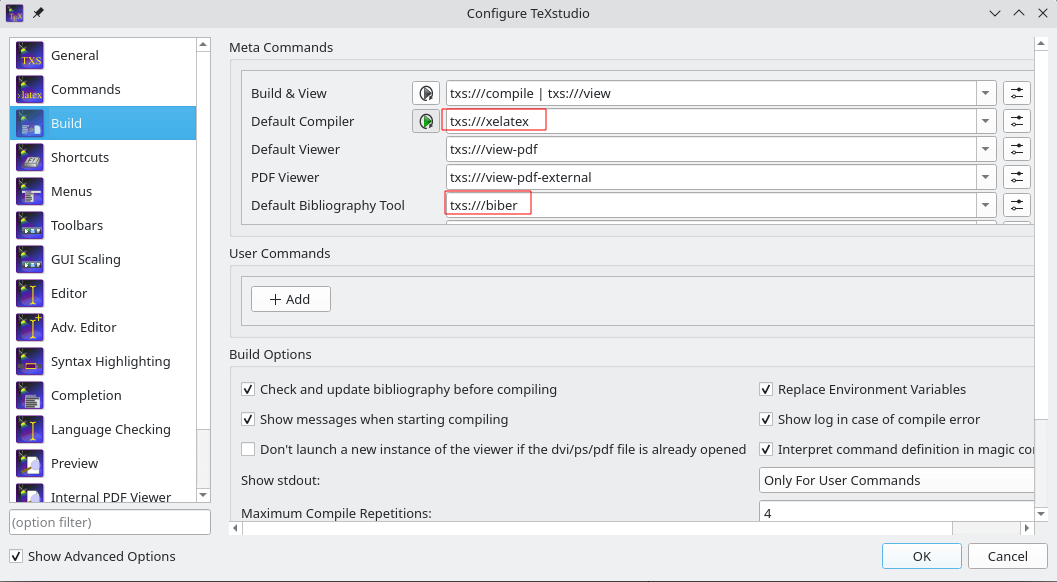
\includegraphics[width=0.8\textwidth]{img/xelatex-biber.png}
    \caption{构建命令选择}
    \label{fig:xelatex-biber}
\end{figure}

同时,代码高亮宏包 minted 需要调用外部命令,进行如 \autoref{fig:xelatex-shell-excape} 所示的设置。

\begin{figure}[H]
    \centering
    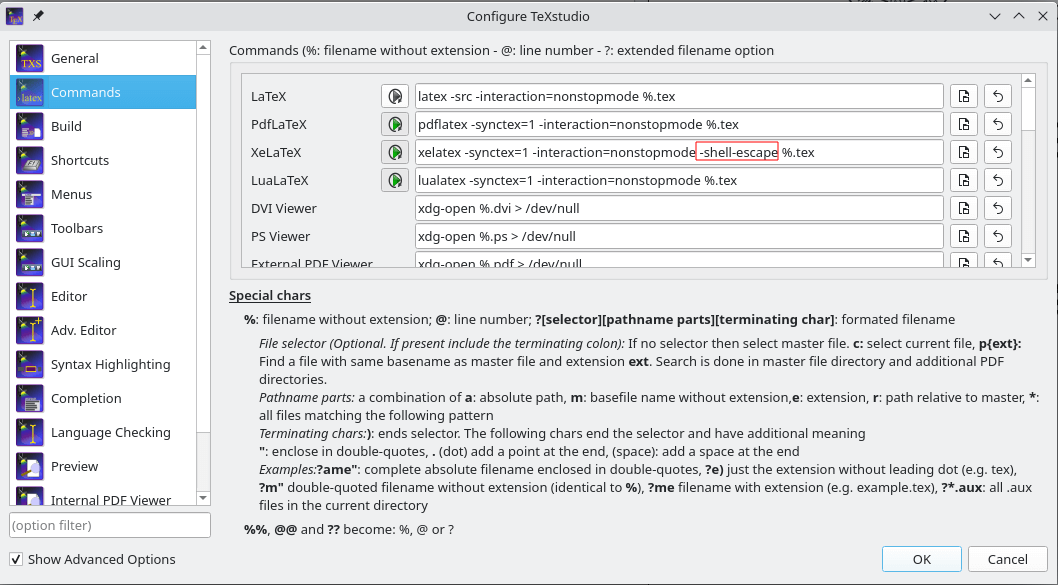
\includegraphics[width=0.8\textwidth]{img/xelatex-shell-escape.png}
    \caption{编译器外部命令设置}
    \label{fig:xelatex-shell-excape}
\end{figure}

\subsection{依赖项}

代码高亮部分使用了 minted 宏包,该宏包依赖 pygmentize(python 库),可以通过如下命令来安装 pygmentize。

\begin{minted}[]{sh}
pip install Pygments
\end{minted}

如果不需要该宏包的话,则在 scutthesis.cls 将 \verb|\|RequirePackage{minted} 以及 tex 中相关使用删除即可。
    \chapter{使用教程}

这里简单介绍一下模板的使用,语法部分可以对照相应的 tex 文件以及生成的 pdf 效果来进行参考。

\section{文件说明}

\begin{table}[htbp]
    \centering
    \zihao{5}
    \caption{主要文件说明}
    \label{tab:file-description}
    %\begin{table}[]
\begin{tabular}{@{}cc@{}}
\toprule
文件/目录      & 说明           \\ \midrule
algo/          & 伪代码          \\
code/          & 代码           \\
content/       & 各章节的内容       \\
img/           & 图片           \\
table/         & 表格           \\
main.tex       & 入口文件         \\
ref.bib        & 参考文献的 bib 文件 \\
scutthesis.cls & 模板           \\ \bottomrule
\end{tabular}
%\end{table}
\end{table}

\section{表}

\LaTeX 的表格语法比较复杂,可以使用某些可视化工具,如 \href{https://www.tablesgenerator.com/}{Table Generator},在线生成 \LaTeX 表格代码后,粘帖到 tex 文件。

\autoref{tab:test} 是一个简单的表格示例。

\begin{table}[htbp]
    \centering
    \zihao{5}
    \caption{一个简单的表格}
    \label{tab:test}
    
\begin{tabular}{c|c|c}
\hline
      & 算法 1 & 算法 2 \\ \hline
数据集 1 &      &      \\ \hline
数据集 2 &      &      \\ \hline
\end{tabular}

\end{table}

\section{图}

封面的 logo 图如 \autoref{fig:logo} 所示。

\begin{figure}[htbp]
    \centering
    \caption{封面的 logo}
    \label{fig:logo}
    
\includegraphics[width=0.4\textwidth]{img/logo.png}
\end{figure}

子图的排版使用的是 subfig 宏包,如 \autoref{fig:subfigure-a} 是 \autoref{fig:subfigure} 中的一个子图。

\begin{figure}[htbp]
    \centering
    \subfloat[子图 a\label{fig:subfigure-a}]{
        
\includegraphics[width=0.2\textwidth]{img/logo.png}
    }
    \subfloat[子图 b\label{fig:subfigure-b}]{
        
\includegraphics[width=0.2\textwidth]{img/logo.png}
    }
    \subfloat[子图 c\label{fig:subfigure-c}]{
        
\includegraphics[width=0.2\textwidth]{img/logo.png}
    }
    \\
    \subfloat[子图 d\label{fig:subfigure-d}]{
        
\includegraphics[width=0.2\textwidth]{img/logo.png}
    }
    \subfloat[子图 e\label{fig:subfigure-e}]{
        
\includegraphics[width=0.2\textwidth]{img/logo.png}
    }
    \subfloat[子图 f\label{fig:subfigure-f}]{
        
\includegraphics[width=0.2\textwidth]{img/logo.png}
    }
    \caption{多个图}
    \label{fig:subfigure}
\end{figure}

在图片的绘制上,
如果是数据统计图,可以使用 Python / Matlab 等工具绘制并保存为 pdf 格式(矢量图);
对于简单的结构图,可以使用 \href{https://www.diagrams.net/}{diagrams.net} 这种绘图工具,保存为 pdf,记得把绘图信息内嵌进去,方便写编辑图片。

\section{算法}

\subsection{伪代码}

伪代码部分,使用了 algorithm 和 algorithmic 两个宏包,伪代码的效果如 \autoref{algo:test} 所示。

\begin{algorithm}[htbp]
    \centering
    \caption{伪代码示例}
    \label{algo:test}
    \begin{algorithmic}[1]
    \REQUIRE Data $x$
    \ENSURE Label $y$
    \STATE Show condition statement;
    \IF {condition}
        \STATE Do something;
    \ENDIF
    \IF {condition}
        \STATE Do something;
    \ELSE
        \STATE Do something;
    \ENDIF
    \IF {condition 1}
        \STATE Do something;
    \ELSIF {condition 2}
        \STATE Do something;
    \ELSE
        \STATE Do something;
    \ENDIF
    \STATE Show loop statement;
    \FOR{ $i=1$ to $n$ }
        \STATE $i \leftarrow i + 1$;
        \STATE Do something;
    \ENDFOR
    \FORALL{$i=1$ to $n$}
        \STATE Do something;
    \ENDFOR
    \WHILE{$i < n$}
        \STATE Do something;
    \ENDWHILE
    \REPEAT
        \STATE Do something;
        \STATE $i \leftarrow i + 1$;
    \UNTIL{$i > n$}
    \LOOP
        \STATE Do something;
    \ENDLOOP
    \STATE Symbol: \NOT, \AND, \OR, \XOR, \FALSE, \TRUE
    \RETURN $y$
\end{algorithmic}

\end{algorithm}

\subsection{代码}

代码高亮部分使用了 minted 宏包,minted 主要有文件内和外部文件两种。
文件内直接在 tex 写皆可,外部文件则是由 tex 引入外部代码文件。

下面是一个文件内的 Python 代码:
\begin{minted}[]{python}
print('Hello World')
\end{minted}

如下为一段简单的 C++ 代码。
\inputminted{c++}{code/test.cpp}

\section{数学公式}

行内公式:$a_n = a_{n-1} + 1$

\autoref{eq:test} 是一个有编号公式。
\begin{equation}
    \label{eq:test}
    a_n = a_{n-1} + 1
\end{equation}

无编号公式:
$$
    a_n = a_{n-1} + 1
$$

有时候,数学符号忘记怎么打了,可以在 \href{http://detexify.kirelabs.org/classify.html}{Detexify} 上面写符号,它会自动生成近似的 \LaTeX 符号代码。

\section{数学环境}

\section{化学}

\subsection{化学式与方程式}


\ce{2H2 + O2 ->T[燃烧] 2H2O}

\ce{N2 + 3H2 <=>T[高温、加压][催化剂] 2NH3}

\ce{^{227}_{90}Th+}

\ce{KCr(SO4)2 * 12H2O}

\ce{C6H5-CHO}

\ce{X=Y#Z}

\section{单位}

这一个部分使用 siunitx 宏包,例如 \SI{1.5}{cm^3/min}、\SI{}{\degreeCelsius}。

\section{引用}

\subsection{论文}

这部分使用了 biblatex 宏包。

引用有两种,上标的\upcite{he2016deep}和非上标的\cite{he2016deep}。
有时候需要多篇引用,例如 \cite{he2016deep, krizhevsky2012imagenet, vaswani2017attention},
根据场景决定是否采用上标形式 \upcite{he2016deep, krizhevsky2012imagenet, vaswani2017attention}。

BibLaTex 信息可以通过此操作获得:在 \href{https://scholar.google.com}{Google Scholar} 上面搜索相应的论文,然后点击引用,再选择 BibLaTex 格式,在获得的文本\textbf{进行修改(根据论文要求的格式)}再粘帖到 ref.bib 文件中。

\subsection{图、表等}

这部分使用了 hyperref 宏包,

\section{脚注}

内容 \footnote{脚注内容}。

    \chapterx{总结}
\sectionx{1 \enspace 小节标题}

感谢使用,欢迎提出修改。
    \appendix

\chapter{附录标题}
\label{appendix:A}

附录内容


    \addcontentsline{toc}{chapter}{参考文献}
    \printbibliography[title={参考文献}]

    \chapterx{致谢}

本模板在编写的时候,参考了如下几个模板,对此表示衷心感谢。

\begin{itemize}
    \item \href{https://github.com/TheNetAdmin/zjuthesis}{TheNetAdmin/zjuthesis}
    \item \href{https://github.com/OChicken/SCUT-Bachelor-Thesis-Template}{OChicken/SCUT-Bachelor-Thesis-Template}
\end{itemize}
\end{spacing}

\end{document}